%!TEX root = <../index.tex>

\section{Experimental Results and Discussion}
\label{sec:5}

The experimental results are described, analyzed and concluded in this section. In section \ref{sec:5.1} the statistics of the corpus after preprocessing is showed briefly. Section \ref{sec:5.2} focuses on the effectiveness of the different STS models, i.e. how precise the STS models predicts an articles as related for a given target article. Furthermore, the operational performance of the STS models is reported in section \ref{sec:5.3}. The above three parts concentrate on the first experiment, which is mentioned in section \ref{sec:4.4}. On the next step, the results of the second experiment are reported in section \ref{sec:5.4}. After reporting the results of the both experiments, we discuss the most severe types of errors that an articles which is virtually unrelated is predicted as related for a target article or a cluster of articles which are properly related are never or rarely predicted as related. In conclusion, we summarize the consequence of selection of the STS models and the challenge of the current work. 

\subsection{Analysis of Preprocessing}
\label{sec:5.1}

The input data to feed the preprocessing methods is one of three semantic components of an article: \ititle{}, \isummary{} and \icontent{}. After preprocessing the text in raw string format is converted to a sequence of phrases which consist of $n$ words. For the n-gram model with different value of $n = 1, 2, 3$, we have three different representation forms for every data source, i.e. \ititle{}, \isummary{} or \icontent{}. A vocabulary is generated from all by preprocessing methods converted data for each representation form of each data source. The size of vocabularies indicates the dimension of document-term vectors as well as impacts the complexity and precision of similarity computing. The advantages of a smaller vocabulary are to decrease the complexity of operations of vectors and to avoid the overfitting of the VSMs and the primary disadvantage is that the semantic information is partly dropped due to the ambiguity of tokens. On the other hand, a larger vocabulary do not lose information, but leads to higher cost of time and memory usage and weaker semantic relevance that the similar meaning is more likely to have quiet different representations. 

\begin{figure}[!htb]
    \centering
    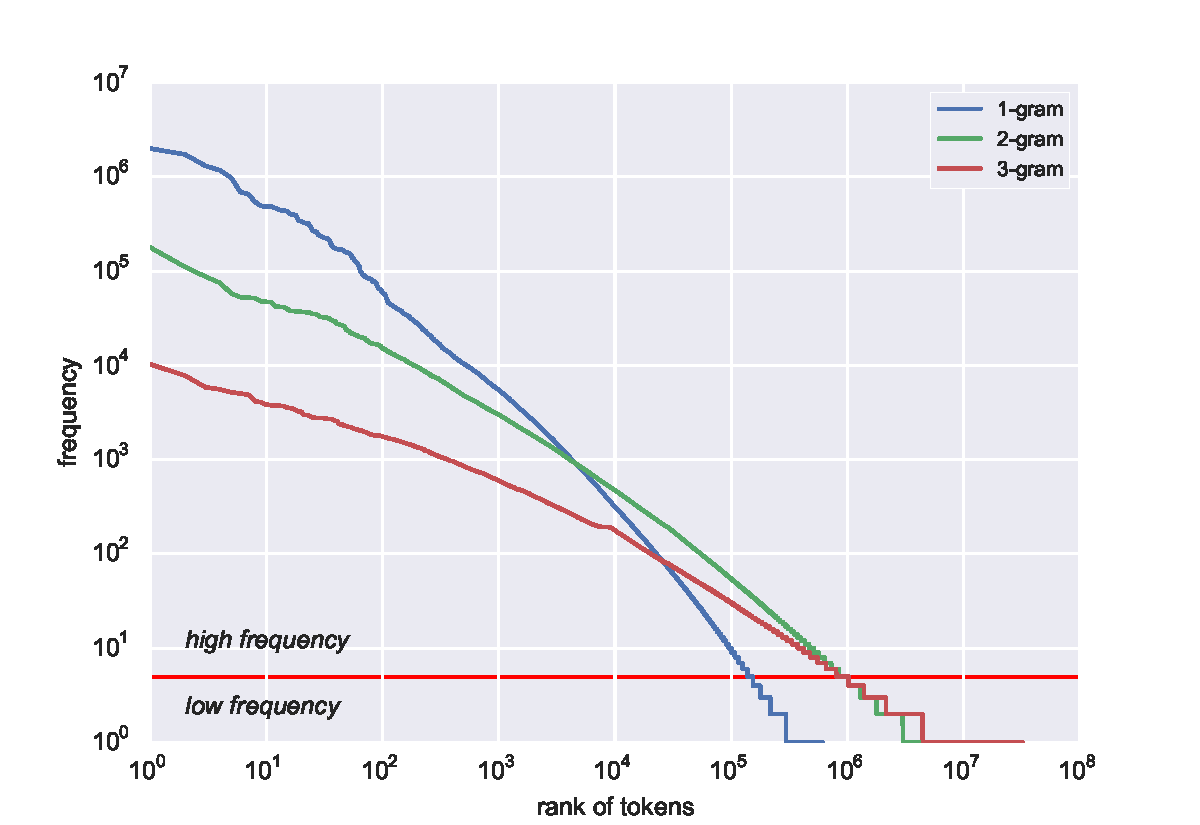
\includegraphics[width=0.8\textwidth]{fig/freqdist}
    \caption{Occurrence Frequency of terms in the corpus for uni-, bi- and trigram in descend ranking. The corresponding preprocessing is \iSE{} and the data source is \icontent{}.}
    \label{fig:freqdist}
\end{figure}

In the n-gram models ($n > 1$), many phrases occur quiet rarely or even only one time in the whole corpus. Figure \ref{fig:freqdist}, which depicts a representative sample the distribution of the occurrence frequency, indicates that only a small quantity of tokens occur repetitively in the corpus (25\% for unigram, 10\% for bigram and 3\% for trigram). Taking into account efficiency, the tokens which appear less than $5$ times can be removed from the vocabulary. We denote the original vocabularies as \ifull{} vocabularies and the reduced vocabularies as \icommon{} vocabularies. 


We consider the size of \ifull{} vocabularies and the proportion of frequent tokens as the metrics to evaluate the vocabulary quality. Figure \ref{fig:vocab_size} shows the comparison between the size of \ifull{} and \icommon{} vocabularies which are generated by the preprocessing methods including \iSP{}, \iSE{}, \iST{} and \iSS{} in the different n-gram models ($n=1, 2, 3$) of the three kinds of data source containing \icontent{}, \ititle{} and \isummary{}. In the unigram model, \iSS{} always generates the both smallest vocabularies with the largest proportion of frequent tokens. 

The \textit{full} vocabularies in bigram and in trigram is $10\times$ and $15\times \sim 40\times$ bigger than the vocabularies in unigram respectively. 

\begin{figure}[!htb]
    \centering
    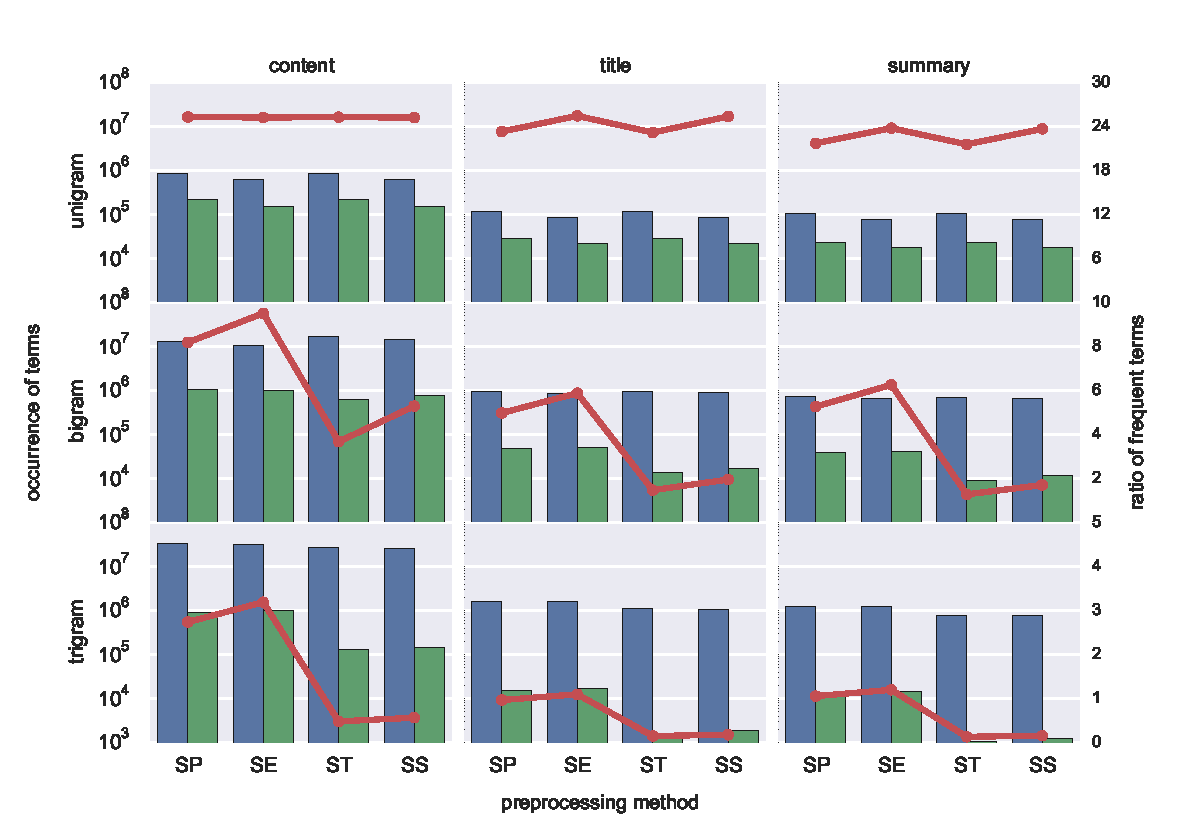
\includegraphics[width=\textwidth]{fig/vocab_size}
    \caption{Comparison the vocabulary size of different preprocessing methods for given data sources with n-gram models. Each column refers to a kind of data source, which is \icontent{}, \ititle{} and \isummary{} respectively while each row refers to a n-gram model: uni-, bi-, and trigram. \textit{Full} vocabularies are illustrated as blue bars and \icommon{} vocabularies as green bars. The red line shows the ratio of the size of \icommon{} vocabularies to the corresponding \ifull{} vocabularies. }
    \label{fig:vocab_size}
\end{figure}


\subsection{Effectiveness of STS Models}
\label{sec:5.2}

\subsection{Efficiency of STS Models}
\label{sec:5.3}

\subsection{Results of Incremental Updating}
\label{sec:5.4}

\subsubsection{Effectiveness}

\subsubsection{Efficiency}

\subsection{Error Analysis}
\label{sec:5.5}

\subsection{Conclusion}
\label{sec:5.6}
